\documentclass[class=minimal,border=0pt,multi=tikzpicture,varwidth=false]{standalone}
%\def\pgfsysdriver{pgfsys-dvisvgm.def}
\usepackage{amsmath}
\usepackage{tikz}
\usetikzlibrary{math}
\begin{document}
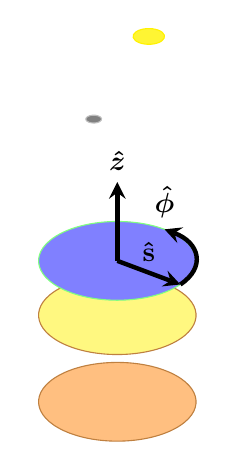
\begin{tikzpicture}[ultra thick,-stealth,
  x={(-0.6cm,-0.4cm)},
  y={( 0.8cm,-0.3cm)},
  z={(   0cm,   1cm)}]
  \draw[color=brown,thin,fill=orange!50!white] (0,0,-1.79) circle [radius=1];
  \draw[color=brown,thin,fill=yellow!50!white] (0,0,-0.69) circle [radius=1];
  \draw[color=green!50!white,thin,fill=blue!50!white] (0,0) circle [radius=1];
  \draw (0,0,0) -- node[above,midway] {$\mathbf{\hat{s}}$} (0,1,0) ;
  \draw (0,1,0) arc [start angle=90, end angle=180, radius=1]
    node[above] {$\boldsymbol{\hat{\phi}}$};
  \draw (0,0,0) -- (0,0,1) node[above] {$\boldsymbol{\hat{z}}$};
  \draw[thin,color=gray!50!white,fill=gray] (0.5,0,2) circle [radius=0.1];
  \draw[thin,color=yellow,fill=yellow!80!white] (0,0.5,3) circle [radius=0.2];
\end{tikzpicture}
\end{document}
